\documentclass[Report.tex]{subfiles}

\newcommand{\newaxis}[4]{
\begin{axis}[
    ybar,
    title={#1},
    ymin=#3, ymax=#4,
    bar width=1em,
    legend style={at={(0.5,-0.25)},anchor=north,legend columns=-1},
    enlarge x limits=0.4,
    x tick label style={align=center,text width=1.7cm},
    symbolic x coords={Logistic Regression, Random Forest, Multi-layer Perceptron},
    xtick=data,
    ylabel={#2}
]
}

\begin{document}

\section{Same player identification}\label{sec:pair-classification}

%There was a subtle issue with the way the binary classification problem was framed in regards to classifying individual games. This led to high accuracies even with only using mouse movement features, as seen in section \ref{sbsec:game-classification}. The issue had to do with the generality of the model. The models were only trained on a relatively small, fixed set of players, making the problem easier to solve as the models only have to learn the behaviour from the players in the set, which does not apply(TODO) to the general Dota 2 playerbase. Furthermore, the classification is only trained on one particular playing and requires the model to be retrained to be able to predict behaviour of another player. This could be extended into a multi-class problem, but it would still be fixed to the small set of players used in training. This leads to the next machine learning approach of \textit{pair} classification.
%In the next and final approach, deals with this issue by framing the player prediction problem in a different way. Rather than ask \textit{Given a game, which player does it belong to?} the problem is framed as \textit{Given a pair of games, do both games belong to the same player?}
% TODO this leads to low testing accuracies?
% TODO results on a lot more players leads to worse accuracy

\subsubsection{Classification on a pair of games}
The goal of this approach is to be able to train on a large mix of players and games, to learn on the features of both games, and predict if it is the same player or not even if many of the players have never been seen before. The idea is to learn the pattern that differentiates between two players. 

To be able to train on pairs of games together, the features had to be altered to fit as single data points. Before, each game was evaluated separately, so every level 3 action in a game could be used. However, in this pair approach, two games must be used together as inputs to the model. Games in general are of different lengths, which causes the number of level 3 actions to be different for every game. Further, the method of generating level 3 actions (section \ref{sec:mm-features}) means even games of the exact same length will not have the same number of these mouse movement actions. The varying number of level 3 actions prevents a straightforward use of them as input to the machine learning model. Instead, statistics such as the mean, standard deviation and range must be used again. The statistics are calculated for each level 3 action feature over the entire game. This causes a lot of data to be lost, as the hundreds or thousands of level 3 actions are reduced to a small number of statistics. Furthermore, recall a majority of features in a level 3 action are already means and standard deviations, so this method is taking an average of a list of averages. To alleviate this issue as much as possible, the games are split into a few portions where each portion has its own statistics. For example, each game can be split into thirds where each third has its own mean, standard deviation and range for each type of level 3 action. Splitting a game this way not only decreases the data loss due to averaging, but enables each portion to be evaluated individually, to see whether any section of a game is more indicative and predictive of player behaviour compared to another section.

\subsection{Mouse movement features}


\begin{figure}[H]
\newcommand{\plotbar}[2]{
\addplot+[
	discard if not={split}{1},
	discard if not={numSplits}{1},
	discard if not={features}{mouse},
] table [x=model, y=#1,col sep=comma] {data/15-pair-cv.csv};
\addlegendentry{#2}
}
\centering
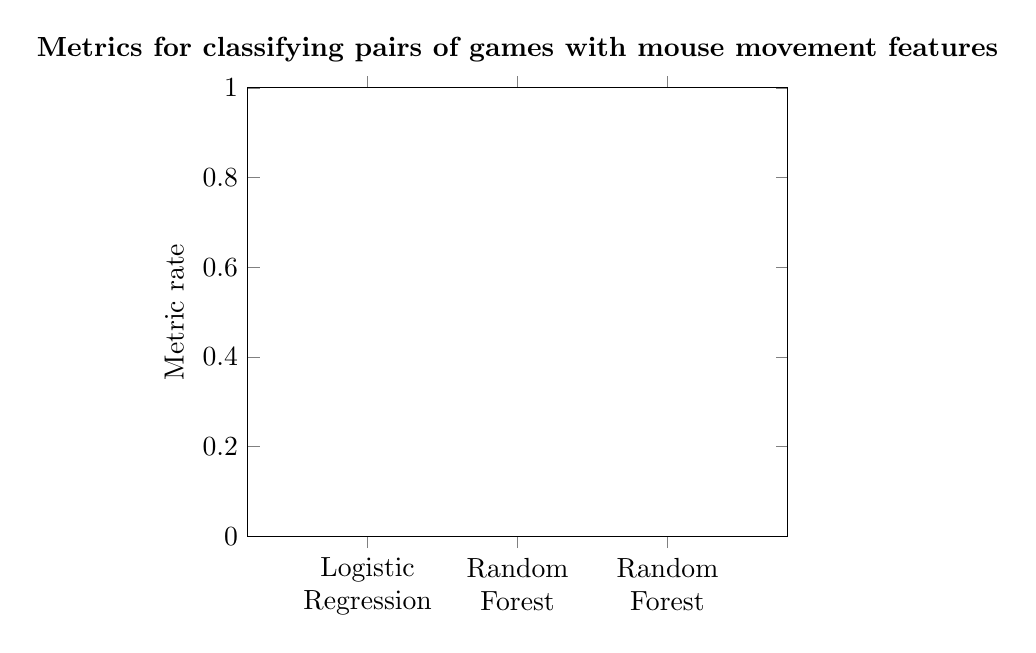
\begin{tikzpicture}
\newaxis{\textbf{Metrics for classifying pairs of games with mouse movement features}}{Metric rate}{0.6}{1.03}

\plotbar{accuracy}{Accuracy}
\plotbar{precision}{Precision}
\plotbar{recall}{Recall}

\end{axis}
\end{tikzpicture}
\end{figure}

\subsection{Game statistic features}

\subsection{Itemisation features}

\subsection{Combined features}
\begin{figure}[H]
\newcommand{\plotbar}[2]{
\addplot+[
	discard if not={split}{1},
	discard if not={numSplits}{1},
	discard if not={features}{#1},
] table [x=model,y=accuracy,col sep=comma] {data/15-pair-cv.csv};
\addlegendentry{#2}
}
\centering
\begin{tikzpicture}
\begin{axis}[
	ybar,
	bar width=1.5em,
	width=11cm,
	legend style={at={(0.5,-0.15)},anchor=north,/tikz/every even column/.append style={column sep=0.5cm}},
	xtick=data,
	enlarge x limits=0.25,
	symbolic x coords={Logistic Regression, Random Forest, Multi-layer Perceptron},
    x tick label style={align=center,text width=2.5cm},
]

\plotbar{mouse}{Mouse movement only}
\plotbar{stats}{Game statistics only}
\plotbar{mouse-stats}{Mouse movement and game statistics}

\end{axis}
\end{tikzpicture}
\caption{Accuracy for pair classification with different features and models.}
\end{figure}


\end{document}

